\chapter{The basis of a class of matrices}
\label{chap:ops}
In this chapter, we look at classes of matrices from a different perspective. Unlike in the previous chapter, where we studied the structure of matrices avoiding a given set of forbidden patterns (usually just one), we are given a class of matrices and a question how the class can be described by forbidden patterns.

Recall that a class of matrices is set of matrices closed under interval minors. While it is obvious that any class of matrices can be described by a set of forbidden patterns, as it suffices to forbid all matrices not contained in the class, it is no longer clear how complex the set can be.

\begin{defn}
Let $\class{M}$ be a class of matrices. The \emph{basis} of $\class{M}$ is a set of all minimal (with respect to minors) matrices $\class{P}$ such that $\class{M}=\Avm{\class{P}}$.
\end{defn}

We show that there are many classes of matrices having a finite basis but there are also classes that have an infinite basis. Let us start with a few simple observations, regarding classes of matrices and their bases. 

\begin{obs}
Let $\class{M}=\Avm{\class{P}}$ for some set of matrices $\class{P}$. Then $\class{M}$ is closed under interval minors.
\end{obs}

\begin{obs}
Every finite class of matrices has a finite basis.
\end{obs}
\begin{proof}
Let $\class{M}$ be a finite class of matrices, let $m$ be the maximum number of rows a matrix from $\class{M}$ has and let $n$ be the maximum number of columns a matrix from $\class{M}$ has. We define a set of matrices~$\class{P}$ to contain all matrices of size smaller or equal to $m\times n$ that do not belong to $\class{M}$ and we add $\{0\}^{m\times(n+1)}$ and $\{0\}^{(m+1)\times n}$. Clearly, $\class{P}$ is finite and $\class{M}=\Avm{\class{P}}$.
\end{proof}

\section{The skew and direct sums}
In the realm of permutations, the skew and direct sums are very useful operations. What follows is a direct generalization to our settings and a few simple results. More interesting statements and the relation with interval minors follow in the next section.

\begin{defn}
For matrices $A\in\Mat$ and $B\in\Pat$ we define their \emph{skew sum} as a matrix $C:=A\dsum B\in\bin^{(m+k)\times(n+l)}$ such that the submatrix~$C[[k+1,m+k],[n]]=A$, $C[[k],[n+1,n+l]]=B$ and the rest is empty. Symmetrically, we define their \emph{direct sum} $D:=A\odsum B\in\bin^{(m+k)\times(n+l)}$ such that $D[[m],[n]]=A$, $D[[m+1,m+k],[n+1,n+l]]=B$. See Figure~\ref{fig:skew}.
\end{defn}

\begin{figure}[!ht]
\centering
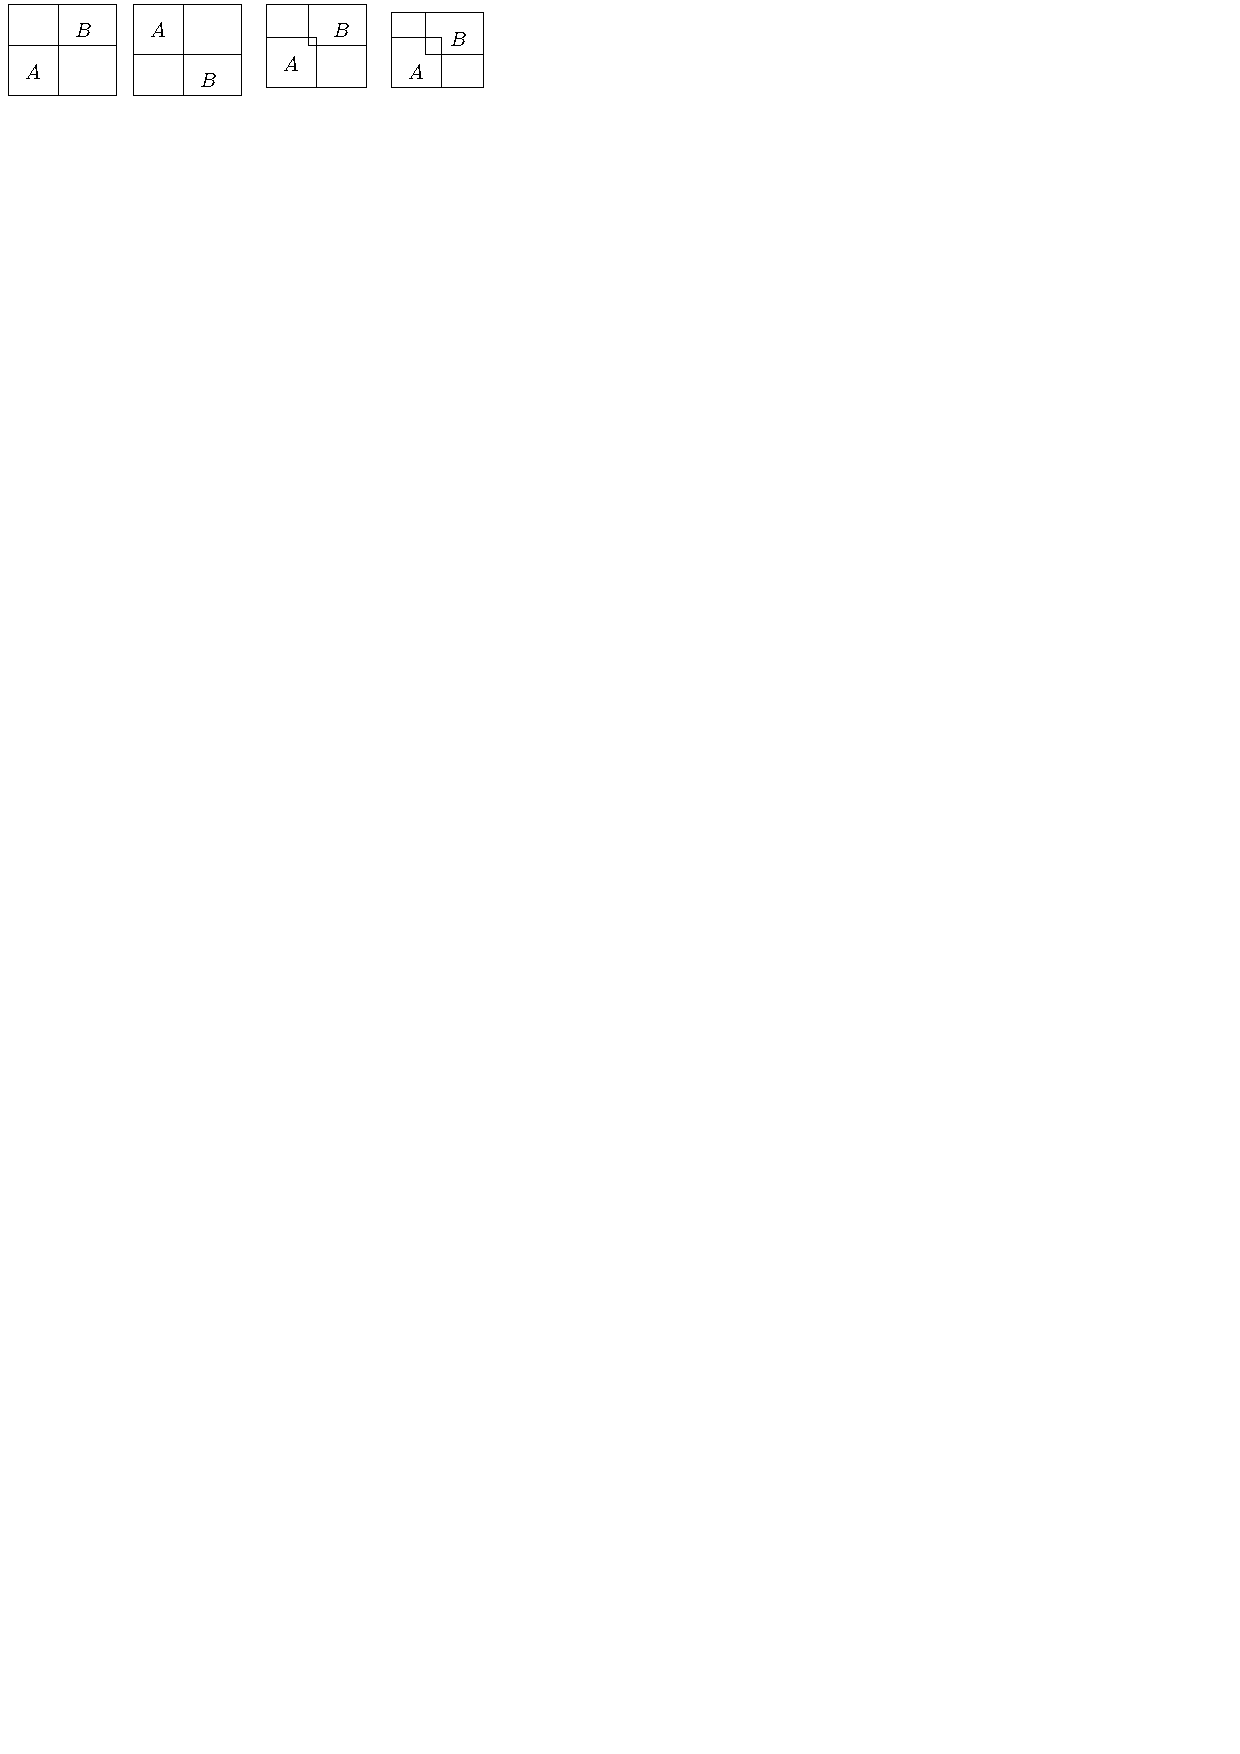
\includegraphics[width=90mm]{img/skew.pdf}
\caption{The skew sum, the direct sum, the skew sum with $1\times1$ overlap and the skew sum with $2\times2$ overlap of matrices $A$ and $B$.}
\label{fig:skew}
\end{figure}

\begin{defn}
For classes of matrices~$\class{A}$ and $\class{B}$ we define their \emph{skew sum} $\class{A}\dsum\class{B}$ as the class of matrices containing the skew sum of all pairs of matrices~$A\in\class{A}$ and $B\in\class{B}$. Symmetrically, we define their \emph{direct sum}.
\end{defn}

Using this notation, we can very easily rewrite the results from the previous chapter. Here is an example of Proposition~\ref{prop:p31} and Proposition~\ref{prop:p33}:

\begin{prop}
$\Avm{\smm{\bullet&\bullet\\\bullet&\circ}}=\Avm{\smm{\bullet&\circ\\\circ&\circ}}\odsum\Avm{\smm{\circ&\bullet\\\bullet&\circ}}$
\end{prop}

\begin{prop}
$\Avm{\smm{\bullet&\bullet\\\bullet&\bullet}}=\left(\Avm{\smm{\bullet&\circ\\\circ&\circ}}\odsum\Avm{\smm{\circ&\bullet\\\bullet&\circ}}\odsum\Avm{\smm{\circ&\circ\\\circ&\bullet}}\right)\cup$

\hspace{54mm}$\left(\Avm{\smm{\circ&\circ\\\bullet&\circ}}\dsum\Avm{\smm{\bullet&\circ\\\circ&\bullet}}\dsum\Avm{\smm{\circ&\bullet\\\circ&\circ}}\right)$.
\end{prop}

Something, we get a great use of later is the closure under the skew sum.

\begin{defn}
For a set of matrices $\class{M}$, let $\Cl{\class{M}}$ denote the smallest class of matrices containing each $M\in\class{M}$ that is closed under the skew sum and interval minors.
\end{defn}

When speaking about interval minors, we suppose, without loss of generality, that the merges of neighboring lines are done after all deletions of one-entries. Similarly, a matrix created from a matrix~$M$ by reapplying the skew sum and taking its interval minor can be also created by taking an interval minor of the skew sum of an appropriate number of copies of $M$.

\begin{obs}
For every set of matrices $\class{P}$, each $M\in\Cl{\class{P}}$ is an interval minor of the skew sum of multiple copies of $P$.
\end{obs}

What follows is a simple example of the relation between the closure under the skew sum and the description using interval minors. We greatly generalize this result in the next section.

\begin{prop}
$\Cl{\smm{\bullet&\circ\\\circ&\bullet}}=\Avm{\smm{\bullet&\circ&\circ\\\circ&\circ&\bullet},\smm{\bullet&\circ\\\circ&\circ\\\circ&\bullet}}$.
\end{prop}
\begin{proof}
The skew sum of an arbitrary number of copies of $\smm{\bullet&\circ\\\circ&\bullet}$ avoids both forbidden patterns and because the relation of being an interval minor is transitive, we have $\Cl{\smm{\bullet&\circ\\\circ&\bullet}}\subseteq\Avm{\smm{\bullet&\circ&\circ\\\circ&\circ&\bullet},\smm{\bullet&\circ\\\circ&\circ\\\circ&\bullet}}$.

From Proposition~\ref{prop:twopatterns}, for every matrix~$M\in\Avm{\smm{\bullet&\circ&\circ\\\circ&\circ&\bullet},\smm{\bullet&\circ\\\circ&\circ\\\circ&\bullet}}$, it holds that for every $r>1$ and $c>1$, if $M[r,c]$ is a one-entry then it either is on the top-left extreme walk~$w$ or both $M[r-1,c]$ and $M[r,c-1]$ are on $w$. Clearly, $\smm{\bullet&\bullet\\\bullet&\bullet}$ is an interval minor of the skew sum of three copies of $\smm{\bullet&\circ\\\circ&\bullet}$ and from the skew sum of multiple copies of $\smm{\bullet&\bullet\\\bullet&\bullet}$, we can create the walk~$w$ and all one-entries outside of it by taking an interval minor.
\end{proof}

%\begin{prop}
%$\Cl{\smm{\bullet&\circ\\\circ&\circ\\\circ&\bullet}}=\Avm{\smm{\bullet&\circ&\circ\\\circ&\circ&\bullet},\smm{\bullet&\circ\\\circ&\circ\\\circ&\circ\\\circ&\bullet},\smm{\bullet&\circ\\\bullet&\circ\\\circ&\bullet},\smm{\bullet&\circ\\\circ&\bullet\\\circ&\bullet}}$.
%\end{prop}

We generalize the skew sum to also allow an overlap between the summed matrices.

\begin{defn}
For matrices $A\in\Mat,\ B\in\Pat$ and integers $a,b$, let $C:=A\dsum_{a\times b}B\in\bin^{(m+k-a)\times(n+l-b)}$ be a matrix such that the submatrix~$C[[k+1,m+k],[n]]=A$, $C[[k],[n+1,n+l]]=B$, the part that overlaps is the elementwise OR of the overlapping submatrices and the rest of $C$ is empty. We say $C$ is the \emph{skew sum with $a\times b$ overlap} of $A$ and $B$. See Figure~\ref{fig:skew}.
\end{defn}

\begin{prop}
\label{prop:smaller}
For integers $a,b,m,n$ such that $a\leq m\leq2a$ and $b\leq n\leq2b$, let $\class{M}$ be an arbitrary set of matrices, not necessarily closed under interval minors, such that:
\begin{itemize}
	\item $\class{M}$ is closed under deletion of one-entries,
	\item $\class{M}$ is closed under the skew sum with $a\times b$ overlap and
	\item there is a $m\times n$ matrix $M\in\class{M}$,
\end{itemize}
then $\class{M}$ is also closed under the skew sum with $(2a-m)\times(2b-n)$ overlap.
\end{prop}
\begin{proof}
Given any $A,B\in\class{M}$ and a matrix~$M\in\class{M}$ such that $M\in\Mat$, let $C=A\dsum_{a\times b}M\dsum_{a\times b}B$. It has the same size as $D=A\dsum_{(2a-m)\times(2b-n)}B$, whose set of one-entries is a subset of one-entries of $C\in\class{M}$; therefore, $D\in\class{M}$.
\end{proof}

We see that with some reasonable assumptions, whenever a set of matrices is closed under the skew sum with an overlap, it is also closed under the skew sum with a smaller overlap. On the other hand, in general, the opposite does not hold even if we work with classes of matrices.

%NOTE: originally this was here to show that while for classes closed under minors a bigger overlap always works (now this is disproved in the following observation) so the question is whether there is any point in having this here anymore.
%\begin{obs}
%There is a set of matrices $\class{M}$ closed under submatrices but not interval minors such that it is closed under the direct sum but it is not closed under the direct sum with $1\times1$ overlap.
%\end{obs}
%\begin{proof}
%Let $\class{M}$ be a class of matrices obtained by applying the direct sum to $\smm{\bullet& \\\ &\bullet}$. Clearly, it is closed under the direct sum. On the other hand, it is not closed under the direct sum with $1\times1$ overlap, as $\smm{\bullet& \\\ &\bullet}\dsum_{1\times1}\smm{\bullet& \\\ &\bullet}=\smm{ &\bullet& \\\bullet& &\bullet\\ &\bullet& }\not\in\class{C}$.
%\end{proof}

\begin{obs}
There is a class of matrices closed under the skew sum with $1\times1$ overlap that is not closed under the skew sum with $2\times2$ overlap.
\end{obs}
\begin{proof}
Let $\class{M}=\Avm{\smm{\bullet& \\ &\bullet}}$. Clearly, $\class{M}$ is hereditary and closed under the skew sum with $1\times1$ overlap. On the other hand, $\class{M}$ is not closed under the skew sum with $2\times2$ overlap, because, for matrices $\smm{\bullet&\bullet\\\bullet& },\smm{ &\bullet\\\bullet&\bullet}\in\class{M}$ it holds $\smm{\bullet&\bullet\\\bullet& }\dsum_{2\times2}\smm{ &\bullet\\\bullet&\bullet}=\smm{\bullet&\bullet\\\bullet&\bullet}\not\in\class{M}$.
\end{proof}

A similar proof shows that for all $a\geq1,b>1$ there is a class of matrices closed under the skew sum with $a\times b$ overlap that is not closed under the skew sum with $(a+1)\times b$ (or $a\times(b+1)$) overlap. Luckily for us, this does not hold for $a=0$ or $b=0$:

\begin{prop}
\label{prop:0to1}
Every class of matrices is closed under the skew sum $\Leftrightarrow$ it is closed under the skew sum with $1\times1$ overlap.
\end{prop}
\begin{proof}
\begin{itemize}
	\item[$\Rightarrow$] If a class is closed under the skew sum then, because it is also closed under interval minors, it is closed under the skew sum with $1\times1$ overlap.
	\item[$\Leftarrow$] Let $\class{M}$ be a class closed under the skew sum with $1\times1$ overlap. Using the assumption that $\class{M}$ is non-trivial, it contains matrices $M_1\in\bin^{2\times1}$ and $M_2\in\bin^{1\times2}$. For $M=M_1\dsum_{1\times1}M_2$, we have $M\in\class{M}$ and we can use Proposition~\ref{prop:smaller} to show $\class{M}$ is closed under the skew sum. \qedhere
\end{itemize}
\end{proof}

\section{Articulations}
Our next goal is to show that the closure under the skew sum of a single matrix creates a class with finite basis. In order to prove it, we define and get familiar with articulations.

\begin{defn}
Let $M\in\Mat$ be a matrix. An element $M[r,c]$ is an \emph{articulation} if it is top-left empty ($M[[r-1],[c-1]]$ is empty) and bottom-right empty ($M[[r+1,m],[c+1,n]]$ is empty). We say that an articulation $M[r,c]$ is \emph{trivial} if $(r,c)\in\{(m,1),(1,n)\}$.
\end{defn}

\begin{obs}
\label{obs:keep}
Let $M$ be a matrix. If there are integers $r,c$ such that the entry~$M[r,c]$ is an articulation, then for every matrix~$P$ such that $P\im M$, if $P[r',c']$ can be mapped to a block containing $M[r,c]$ then $P[r',c']$ is an articulation.
\end{obs}

\begin{defn}
A matrix~$P_1$ is a \emph{proper} interval minor of a matrix~$P$, if $P_1\im P$ and $P_1\neq P$. We say that the matrix~$P$ is \emph{decomposable} if there exist $P_1,P_2$ proper interval minors of $P$ such that $P=P_1\dsum_{1\times1}P_2$; otherwise, $P$ is \emph{indecomposable}.
\end{defn}

\begin{obs}
\label{obs:art}
Let $P\in\Pat$ be a matrix. The matrix~$P$ is indecomposable $\Leftrightarrow P$ has no non-trivial articulation and both its trivial ones are empty.
\end{obs}

\begin{lemma}
\label{lemma:rel}
Let $\class{M}$ be a class of matrices and let $\class{P}$ be its basis. The class~$\class{M}$ is closed under the skew sum with $1\times1$ overlap $\Leftrightarrow$ every $P\in\class{P}$ is indecomposable.
\end{lemma}
\begin{proof}
\begin{itemize}
	\item[$\Rightarrow$] Let $P\in\class{P}$ be a decomposable pattern and let $P_1,P_2$ be proper interval minors of $P$ such that $P=P_1\dsum_{1\times1}P_2$. While $P_1,P_2\in\Avm{\class{P}}$, we have $P\not\in\Avm{\class{P}}=\class{M}$.
	\item[$\Leftarrow$] Let there be matrices $M_1,M_2\in\Avm{\class{P}}$ such that there is a pattern~$P\in\class{P}$ of size $k\times l$ for which $P\im M=M_1\dsum_{1\times1}M_2$. Since $P\nim M_1$ and $P\nim M_2$, the pattern~$P$ contains a non-trivial articulation or one of its trivial articulations is a one-entry and from Observation~\ref{obs:art}, the pattern~$P$ is decomposable. \qedhere
\end{itemize}
\end{proof}

In what follows, we always assume that all articulations are on a reverse walk (no two articulations form $\smm{\bullet& \\ &\bullet}$) and a matrix between two articulations $M[r_1,c_1]$ and $M[r_2,c_2]$ is the matrix $M[[r_2,r_1],[c_1,c_2]]$.

\begin{lemma}
\label{lemma:artic}
Let $\class{P}$ be a set of matrices, then for all matrices $M\in\Mat$ it holds that $M\in\Cl{\class{P}}\Leftrightarrow$ there exists a sequence of articulations of $M$ on a reverse walk such that for each matrix~$M'$ in between two consecutive articulations there exists a pattern~$P\in\class{P}$ such that $M'\im\smm{1}\dsum P\dsum\smm{1}$.
\end{lemma}
\begin{proof}
\begin{itemize}
	\item[$\Rightarrow$] Having Proposition~\ref{prop:0to1} in mind, consider the skew sum with $1\times1$ overlap of multiple copies of elements of $\class{P}$ and consider the sequence of articulations containing an articulation between each pair of consecutive copies of matrices from $P$, and the trivial articulations~$M[m,1]$ and $M[1,n]$.
	
	Between each pair of consecutive articulations, we have a matrix from $\class{P}$ with potentially new one-entries in the top-right and bottom-left corners, and so the statement holds. When we take an arbitrary interval minor and keep original articulations, each matrix between two consecutive articulations is an interval minor of $\smm{1}\dsum P\dsum\smm{1}$ for the corresponding $P\in\class{P}$.
	\item[$\Leftarrow$] We can simply blow up each matrix~$M'$ between two consecutive articulation to the skew sum of three copies of the corresponding matrix $P$ and because $M'\im\smm{1}\dsum P\dsum\smm{1}\im P\dsum P\dsum P$ it holds $M\in\Cl{\class{P}}$. \qedhere
\end{itemize}
\end{proof}

Finally, we show that the closure under the skew sum of a single matrix can always be described by a finite number of forbidden patterns.

\begin{thm}
For all matrices~$M\in\Mat$, $\Cl{M}$ has a finite basis.
\end{thm}
\begin{proof}
Let $\class{F}$ be the basis of $\Cl{M}$. We need to prove that $\class{F}$ is finite. Thanks to Proposition~\ref{prop:0to1}, $\Avm{\class{F}}=\Cl{M}$ is closed under the skew sum with $1\times1$ overlap and from Lemma~\ref{lemma:rel} follows that every $F\in\class{F}$ is indecomposable. We denote by $\class{P}$ the set of matrices $F\in\class{F}$ such that $F$ has at most $3m+2$ rows and $3n+2$ columns. We want to show $\Cl{M}=\Avm{\class{P}}$.
\begin{itemize}
	\item[$\subseteq$] Clearly, $\class{P}$ is finite and we immediately see that $\Cl{M}\subseteq\Avm{\class{P}}$.
	\item[$\supseteq$] For contradiction, consider a minimal (with respect to interval minors) matrix $X\in\Avm{\class{P}}\smallsetminus\Cl{M}$. There are no $X_1,X_2$ proper interval minors of $X$ such that $X=X_1\dsum_{1\times1}X_2$; otherwise, as $X_1,X_2\in\Avm{\class{P}}$ and $X$ is the minimum matrix such that $X\not\in\Cl{M}$, we would have $X_1,X_2\in\Cl{M}$; therefore, $X\in\Cl{M}$ and a contradiction.

Without loss of generality, we assume $X\in\Pat$ has at least $3n+3$ columns. Let $X'$ denote a matrix created from $X$ by deletion of the first row. We have $X'\in\Avm{\class{P}}$ and from minimality of $X$ also $X'\in\Cl{M}$. From Lemma~\ref{lemma:artic}, there is a sequence of articulations of $X'$ on a reverse walk such that each matrix between two consecutive articulations is an interval minor of $\smm{1}\dsum M\dsum\smm{1}$. Let $X'[r,c]$ be the first articulation from the sequence (sorted by columns in ascending order) for which $c>1$. The matrix between $X'[r,c]$ and the previous articulation in the sequence is an interval minor of $\smm{1}\dsum M\dsum\smm{1}$, which also means that $c\leq n+2$. Since $X[r,c]$ is not an articulation, it must hold that $X[1,c_1]=1$ for some $c_1<c\leq n+2$. Symmetrically, let $X''$ denote a matrix created from $X$ by deletion of the last row. Following the same steps, we consider the last articulation $X''[r',c']$ such that $c'<l$ and have that $c'\geq l-n-1$. Since $X[r',c']$ is not an articulation, it must hold that $X[k,c_2]=1$ for some $c_2>c'\geq l-n-1\geq 3n+3-n-1=2n+2$. Therefore, there are at least $n-1$ columns between $X[1,c_1]$ and $X[k,c_2]$.

We showed that a matrix~$Y\in\bin^{2\times(n+1)}$ such that the only one-entries are $Y[1,1]$ and $Y[2,n+1]$ is an interval minor of $X$. To reach a contradiction, it suffices to show that there is a matrix~$P\in\class{P}$ such that $P\im Y$. For contradiction, let $Y\in\Avm{\class{P}}$ and since $Y\im X$ and $X$ is minimum such that $X\not\in\Cl{M}$ it holds $Y\in\Cl{M}$. But this cannot be, because $Y$ contains no non-trivial articulation and from Observation~\ref{obs:keep}, we know that every matrix $Z\in\Cl{M}$ bigger than $m\times n$ contains at least one. \qedhere
\end{itemize}
\end{proof}

\section{Bases}
We recall that the basis of a class of matrices $\class{M}$ is a set of all minimal (with respect to interval minors) matrices $\class{P}$ such that $\class{M}=\Avm{\class{P}}$. It goes without saying that it does not make sense to consider a basis of a set of matrices that is not closed under interval minors.

So far, we showed that whenever $\class{M}$ is finite, its basis is also finite. The same holds when $\class{M}=\Cl{M}$ for any matrix~$M$. We show next, that unlike in graph theory, there are classes of matrices that do not have finite basis. Moreover, we show that even for a class~$\class{M}$ with a finite basis, its closure~$\Cl{\class{M}}$ can have an infinite basis.

\begin{defn}
Let $P$ be a matrix. We denote by $\R{P}$ a set of all minimal (with respect to minors) indecomposable matrices $P'$ such that $P\im P'$. For a set of matrices $\class{P}$, let $\R{\class{P}}$ denote a set of all minimal (with respect to minors) matrices from the set $\bigcup_{P\in\class{P}}\R{P}$.
\end{defn}

\begin{thm}
\label{thm:basis}
Let $\class{M}$ and $\class{P}$ be sets of matrices such that $\class{M}=\Avm{\class{P}}$, then $\Cl{\class{M}}=\Avm{\R{\class{P}}}$.
\end{thm}
\begin{proof}
\begin{itemize}
	\item[$\subseteq$] For contradiction, let $M\in\Cl{\class{M}}\smallsetminus\Avm{\R{\class{P}}}$ be a minimal (with respect to interval minors) matrix. It follows that $M\in\R{\class{P}}$. Then, the matrix~$M$ is indecomposable; therefore, according to Observation~\ref{obs:art}, there is no non-trivial articulations in $M$ and both trivial articulations are empty. According to Lemma~\ref{lemma:artic} and the fact $M$ contains no non-trivial articulation, it holds $M\im\smm{1}\dsum M'\dsum\smm{1}$ for some $M'\in\class{M}$. Because the trivial articulations are empty, it even holds $M\im M'$. We also know $P\im M$ for some $P\in\class{P}$, which together give us a contradiction with $\class{M}=\Avm{\class{P}}$.
	\item[$\supseteq$] First of all, $\Avm{\R{\class{P}}}$ is closed under the skew sum with $1\times1$ overlap. For contradiction, assume there are matrices $M_1,M_2\in\Avm{\R{\class{P}}}$ but $M=M_1\dsum_{1\times1}M_2\not\in\Avm{\R{\class{P}}}$. Then there exists a matrix~$P\in\R{\class{P}}$ such that $P\im M$. Because $P$ is indecomposable, it follows that either $P\im M_1$ or $P\im M_2$ and we have a contradiction.

It suffices to show that the inclusion holds for any matrix $M\in\Avm{\R{\class{P}}}$ that is not a skew sum with $1\times1$ overlap of non-empty interval minors of $M$. From Observation~\ref{obs:art}, we know that $M$ does not contain any non-trivial articulation and those trivial ones are empty. Thus, $M\in\Avm{\class{P}}=\class{M}$ and so $M\in\Cl{\class{M}}$. \qedhere
\end{itemize}
\end{proof}

\begin{cor}
Let $\class{M}$ and $\class{P}$ be sets of matrices such that $\class{M}=\Avm{\class{P}}$, then $\R{\class{P}}$ is the basis of $\Cl{\class{M}}$.
\end{cor}

What follows is a construction of parameterized matrices that become the main tool of finding a class of matrices with an infinite basis.

\begin{defn}
Let $Nucleus_1=\smm{\circ&\bullet&\circ}$ and for $n>1$ let $Nucleus_n$ be a matrix of size ${n\times n+1}$ described by the examples:
\begin{center}
$Nucleus_2=\smm{\bullet&\circ&\circ\\\circ&\circ&\bullet}\ \ 
Nucleus_3=\smm{ &\bullet&\circ& \\\bullet& & &\bullet\\ &\circ&\bullet& }\ \ 
Nucleus_n=\smm{ & & & & & &\bullet&\circ& \\ & & & & &\bullet& & &\bullet\\ & & & &\bullet& & &\bullet& \\ & & &\cdots& & &\bullet& & \\ & &\bullet& & &\cdots& & & \\ &\bullet& & &\bullet& & & & \\\bullet& & &\bullet& & & & & \\ &\circ&\bullet& & & & & & \\}$.
\end{center}
\end{defn}

\begin{defn}
Let $Candy_{k,n,l}$ be a matrix given by $I_k\dsum_{1\times2}Nucleus_n\dsum_{1\times2}I_l$, where $I_k,I_l$ are unit matrices of sizes $k\times k$ and $l\times l$ respectively.
\end{defn}
$Candy_{4,1,4}=\smm{
 & & &\bullet& & & \\
 & & & &\bullet& & \\
 & & & & &\bullet& \\
\bullet& &\circ&\bullet&\circ& &\bullet\\
 &\bullet& & & & & \\
 & &\bullet& & & & \\
 & & &\bullet& & & }$
$Candy_{4,4,4}=\smm{
 & & & & &\bullet& & & \\
 & & & & & &\bullet& & \\
 & & & & & & &\bullet& \\
 & & & & \bullet&\circ& & &\bullet\\
 & & &\bullet& & &\bullet& & \\
 & & \bullet& & &\bullet& & & \\
\bullet& & &\circ&\bullet& & & & \\
 &\bullet& & & & & & & \\
 & &\bullet& & & & & & \\
 & & &\bullet& & & & & }$

\begin{thm}
\label{thm:inf}
There exists a matrix $P$ for which $\R{P}$ is infinite.
\end{thm}
\begin{proof}
Let $P=Candy_{4,1,4}$. For all $n>3$ it holds $P\im Candy_{4,n,4}$ and it suffices to show that each $Candy_{4,n,4}$ belongs to the basis of $\Avm{P}$ and it is indecomposable. According to Observation~\ref{obs:art}, the second condition holds as $Candy_{4,n,4}$ contains no non-trivial articulation and the trivial ones are empty. To show it belong to the basis, we need to consider any matrix~$M\im Candy_{4,n,4}$ such that $M\neq P$ and argue that either $P\nim M$ or $M$ is decomposable.

Thanks to Observation~\ref{obs:keep}, when we find a non-trivial articulation~$M[r,c]$ such that $M[[r,k],[c]],M[[r],[c,l]]$ are non-empty, it stays there in any interval minor, because we cannot delete one-entries $M[1,n-3],M[2,n-2],M[3,n-1]$ and $M[4,n]$ (and symmetrically $M[m-3,1],M[m-2,2],M[m-1,3],M[m,4]$) without losing the condition $P\im M$. Therefore, we can only consider one minoring operation at a time.

It is easy to see that when a one-entry is delete, then the matrix does not belong to $\R{P}$ anymore. Consider that rows $r$ and $r+1$ are merged to one with the elementwise OR. If $r<4$ or $r>n+2$ then $P$ is no longer an interval minor of such matrix. Otherwise, the original $Candy_{4,n,4}[r,n-r+2]$ becomes an articulation. Symmetrically, the same holds for columns.
\end{proof}

\begin{cor}
There exists a class of matrices $\class{M}$ having a finite basis such that $\Cl{\class{M}}$ has an infinite basis.
\end{cor}
\begin{proof}
From Theorem~\ref{thm:inf}, we have a matrix $P$ for which $\R{P}$ is infinite. Class $\class{M}=\Avm{P}$ has a finite basis. On the other hand, from Theorem~\ref{thm:basis}, we have $\Cl{\class{M}}=\Avm{\R{P}}$.
\end{proof}